\section{\label{sec:back:mc}\Glsfmtname{mc}/\glsfmtname{ps}}

\emph{\Gls{mc}}, also known as \emph{\gls{ps}} (the two terms are generally used interchangeably), is a bio-inspired model of computing created by Gheorghe Păun in the late 1990s \cite{tPaun98a,Paun2000}.  It was originally conceived of by considering the process of chemical reactions and exchanges that occur inside living biological cells and between the membranes therein, and regarding this process as a form of computation.  \Gls{mc} was identified in 2016 by the National Research Council of Canada as \textcquote[][p. 17]{Wiseman2016}{a rigorous and comprehensive framework that provides a parallel distributed framework with flexible evolution rules.}

\citeauthor{Paun2002} describes \gls{mc} as:
\blockcquote[][p.~VII]{Paun2002}{Membrane computing is a branch of natural computing which abstracts from the structure and the functioning of living cells. In the basic model, the membrane systems -- also called P systems -- are distributed parallel computing devices, processing multisets of objects, synchronously, in the compartments delimited by a membrane structure. The objects, which correspond to chemicals evolving in the compartments of a cell, can also pass through membranes. The membranes form a hierarchical structure --- they can be dissolved, divided, created, and their permeability can be modified. A sequence of transitions between configurations of a system forms a computation. The result of a halting computation is the number of objects present at the end of the computation in a specified membrane, called the output membrane. The objects can also have a structure of their own that can be described by strings over a given alphabet of basic molecules - then the result of a computation is a set of strings.}

\begin{figure}
    \centering
    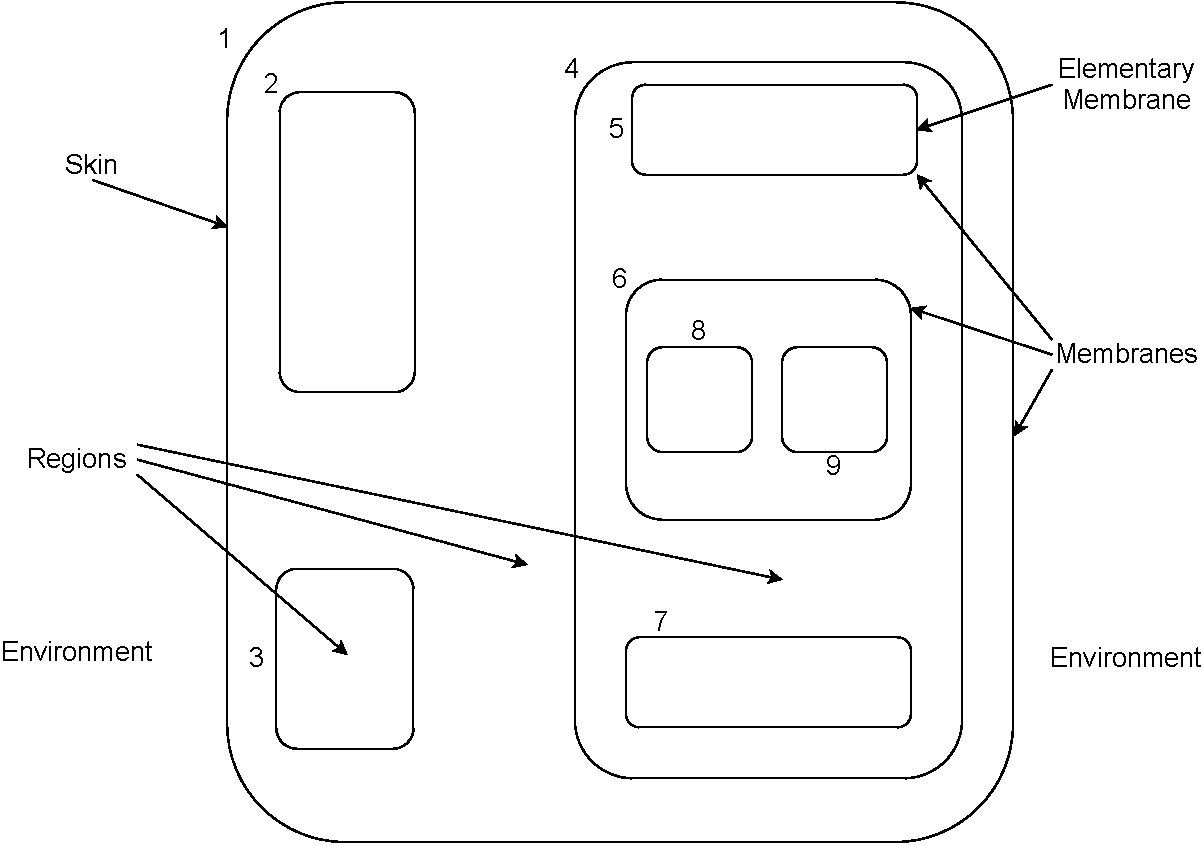
\includegraphics[width=1.0\textwidth]{chapters/background/images/membranestructure.pdf}
    \caption[Diagram illustrating the basic membrane structure as introduced by Păun]{Diagram illustrating the basic membrane structure as introduced by Păun (reproduced from Figure 1 in \cite{Paun2006}).  The outermost membrane is referred to as the \emph{skin}, and membranes without membranes nested inside them as \emph{elementary membranes}.  Each membrane is numbered with a label, written near its border}
    \label{fig:back:membranestructure}
\end{figure}

\Gls{ps} works analogously to a typical modern electronic computer, in that the system stores data and processes \& updates those data based on a predefined program, with a view to arriving at a computable answer based on the starting state and any inputs to the system \cite{Paun2002,Paun2010b}.  In classical \gls{ps}, the data are multisets of symbols, representing various chemicals and their quantities.  These are found inside one or more \emph{cells},\footnote{Loosely based on real biological cells.} which form a hybrid between main memory and the processing units of a computer.  The instructions of the program itself are provided by \emph{rules}, which specify transformations of objects and interactions with the surrounding environment and other membranes or cells.  \Cref{fig:back:membranestructure} is a diagram showing the basic structure of a traditional \glspl{ps} according to Păun's early conception.

There are now, broadly, three main families of \gls{ps} variants:  \emph{\gls{clps}} \cite{Paun2001,Paun2002}, \emph{\gls{tlps}} \cite{tMaPaPaRo01a,Martin-Vide2003} and \emph{\gls{snps}}\footnote{\Gls{snps} have lately been brought under the umbrella of \emph{neural-like \gls{ps}}.  This only occurred near the end of preparation of the present dissertation, however, and the subfield is still completely dominated by \gls{snps}.  Therefore, this dissertation henceforth refers solely to \gls{snps}.}  \cite{Ionescu2006}.\footnote{Other \gls{ps} variants have been created, but most are now used infrequently, if ever.  Most recent work in \gls{mc} has focused on sub-variants of \gls{clps}, \gls{tlps}, \gls{snps} and \gls{cps}.}  \Gls{clps} is the direct descendant of the original classical \gls{ps}, and sees objects compartmented into \emph{membranes}, which are arranged in a graphical tree structure with the outermost \emph{skin} membrane -- which separates the cell from its \emph{environment} -- as the root of the tree.  In most variants, objects can evolve inside a membrane, but also be communicated between membranes (and the environment).  Furthermore, membranes can \emph{divide} or \emph{dissolve} themselves, and may have one or more special properties, such as \emph{polarization} \cite{Paun1999a}.

On the other hand, \gls{tlps} and \gls{snps} both arrange their computing \glspl{compartment} -- named \emph{cells} or \emph{neurons}, respectively -- as nodes in arbitrary digraphs, with the edges between them representing connecting channels or synapses.  Whereas \gls{clps} emphasises the evolution of multisets of objects inside membranes of a given cell, \gls{tlps} and \gls{snps} emphasise communication between separate cells/neurons, and might not include any capacity for internal evolution inside cells.  If new objects are required, they are imported via communication with the environment, which possesses an unlimited number of all objects but has no rules of its own.

While \gls{tlps} have arbitrary alphabets, only one object is used in \gls{snps}, the \emph{spike}.  This means that \gls{tlps} frequently are much like \gls{clps} in that they have custom objects for each purpose, with the key difference usually being in the arrangement of the \glspl{compartment} relative to each other and the choice between the two motivated primarily by which one better fits the computation to be modelled.

Conversely, \gls{snps} represent everything through the use of differing quantities of the spike, kept in different neurons.  This means that it can be more complex to model certain problems, but also arguably means that \gls{snps} are, \textit{prima facie}, closer to Lambda Calculus \cite{Barendregt1984} and Church Numerals (see \eg{} \cite{Koopman2014,Hinze2005}), as well as Register Machines (see \eg{} \cite{Korec1996}) (and indeed Register Machines have been simulated with \gls{snps} \cite{Pan2010}).  All three main types of \gls{ps}, in some form, have been proven Turing-universal though \cite{Bernardini2005,Chen2008,Freund2005}, so all three should be capable of expressing the same computations in different forms.  Furthermore, because \gls{snps} can be easily represented numerically, they lend themselves well to vector/matrix representations \cite{Zeng2010,Martinez-del-Amor2021,Gheorghe2021,Hu2016}.  This means that, potentially, \gls{snps} implementations can take advantage of high-performance techniques such as directly using BLAS\footnote{\url{https://www.netlib.org/blas/}} \& LAPACK\footnote{\url{https://www.netlib.org/lapack/}} and/or \glspl{gpu} \cite{Aboy2019}.

Arguably, the most noteworthy and important aspects of \gls{ps} models are that:
\begin{inparaenum}[(i)]
\item They have no space limit.  That is, they contain an unbounded number of cells, objects, and membranes;
\item Usually, across all \glspl{compartment}, all rules that can be applied are applied, as many times as possible given the current number of objects available.
\end{inparaenum}
These two features mean that \gls{ps} have unbounded space and processing capacity, which can be used to solve traditionally computationally difficult problems relatively quickly \cite{Sosik2003,Jimenez2003,Paun1999a,Henderson2020}.  Most of these solutions, however, rely on trading time complexity for space complexity.  While this works in the theoretical framework, electronic simulations of the systems do not have access to unlimited instantaneous memory space, so fast solutions may be impractical with current real-world computers.

\citeauthor{Valencia-Cabrera2019} said of this:
\blockcquote[][p.~213]{Valencia-Cabrera2019}{We do not know if we will have those machines able to solve NP-complete problems in polynomial time, in many cases even linear time, but \textins{that does} not necessarily mean we will have to wait until that moment in biochemical technology to find some relevant use of P systems. As Babbage kept working on his ideas, not simply waiting until the precise moment when Turing, Von Neumann, and their contemporaries witnessed the first electronic computers based on similar principles, membrane computing must keep moving, finding new ways to provide a step further.}

Nevertheless, modelling a problem in \gls{mc} can lead to new insights or improved formulations of solutions, as occurs in \cref{chap:nmp}.  For example, in \cite{GimelFarb2013a} (building on \cite{Gimelfarb2011}) \citeauthor{GimelFarb2013a} describe how formulating symmetric dynamic programming \gls{sm} in terms of \gls{ps} enabled them to find a bug in the implementation, \textcquote[][p.~24]{GimelFarb2013a}{but also (and what is much more important) refactor this algorithm, based on our cell structure.  The result is a more robust and flexible version, which allows us to fine tune its parameters and enhance its capabilities, without rewriting it from scratch.}  Furthermore, as reported in \cite{Nicolescu2014b}, this exercise led directly to the creation of a new \gls{sm} algorithm, concurrent propagation \cite{Gimelfarb2012}.  \citeauthor{Pang2018} \cite{Pang2018} also claim significant benefits from modelling certain problems in a novel variant of \gls{enps} \cite{Pavel2010}, but it is unclear how much of the stated benefit compared to their baseline implementation arises instead from the use of a \gls{gpu}.

\subsection{Objects, Rules and Steps}
All known \gls{ps} types fundamentally operate on a similar basis:  One or more sets of rules -- \emph{\glspl{ruleset}} -- are defined, describing how the \emph{objects} present in the system's \glspl{compartment} change at each \emph{step}.  As mentioned above, the objects are usually multisets of arbitrary symbolic \emph{atoms}, with the exceptions of \gls{snps} which uses the spike as its only symbol, and numerical \gls{ps}, which uses ordinary numbers in place of atoms.  Systems may introduce other object types as required.

\Gls{ps} types normally operate synchronously and assume the presence of a global clock.  At each clock ``tick'', every \gls{compartment} compares its extant objects and its \emph{evolution rules}, determines which rules are applicable given the current objects, and then deletes the objects used in the rules, replacing them with new ones as the rules dictate.  This process comprises a step.  The progressive execution of the system's rules over multiple steps is referred to as the system's evolution.

All \gls{ps} evolve, and therefore all types have evolution rules (though they may not be referred to as such).  Other types of rules are possible, including: \emph{dissolution} and \emph{division} rules in \gls{clps} and \gls{tlps}, where membranes either dissolve and release their objects into their parent membrane, or replicate themselves (essentially performing mitosis) and distribute their contents among the new membranes; \emph{forgetting} rules in \gls{snps} whereby one or more copies of the spike are removed from a given neuron; or, splicing rules in splicing \Gls{ps}\footnote{Particularly notable for working over strings of an alphabet, instead of multisets.} \cite[Ch.~8]{Paun2010b}.

All rules use the same basic model.  At the start of a step, they check if the necessary pre-conditions for the rule are met.  If they are, then any changes to the state of the system specified by the rule occur.  It is common for rules to remove or delete some objects in the relevant \gls{compartment}, and instantiate new ones.  It is typically assumed that all objects are deleted or created instantaneously at the last moment of the rules' execution.

Generally, rules are specified in the form \textsf{\gls{lhs}} \(\rightarrow\) \textsf{\gls{rhs}}, with objects to be removed (the presence of which are therefore a precondition) written in the \gls{lhs} and objects to be created written in the \gls{rhs}.  Unless otherwise specified, it is typically assumed that all rules which can be applied at a given step are applied.

\subsubsection{Weak Priority Order}

Many, perhaps most, types of \gls{ps} \glspl{ruleset} use a \emph{weak-priority} ordering.  This means that some rules will be tested for applicability ahead of others, on some priority basis, but earlier applicable rules only prevent later applicable rules from being applied if there is a conflict between the two.  The most common way that this conflict can arise is by two rules trying to use the same pre-existing object in the \gls{compartment}.

Generally speaking, an individual rule will select one or more copies of one or more objects in the \gls{compartment} for use.  At the end of the rule's application, these objects are deleted and replaced with any new ones the rule specifies.  Since the rule will delete the chosen objects, it would not make sense for another rule to be able also to use and then delete the same objects.  Therefore, the first rule to select (or take hold of or seize \etc{}) a given object prevents any other rule from using it, and thus the first rule has priority over later rules.

The typical method of defining rules' priority is to use \emph{top-down} ordering.  This simply means that the rules presented first in a \gls{ruleset} have priority over those rules presented further down.  The basic process to determine which rules to apply is therefore a sequential one.  Starting with the first rule, and proceeding with each successive rule in turn, test if the rule is applicable at all.  If it is, set it to be applied during the step as many times as possible depending on the rule, the objects present, and the run-time mode (see \eg{} \cref{sec:cps:applicationmodes} for a discussion of this in relation to \gls{cps}).

Any objects now set to be deleted by a previous rule are then unavailable to a later rule, but if there are sufficient remaining objects for that rule to apply, it still may, giving a \emph{weak} priority to the earlier rules.  The application of an earlier rule does not guarantee that a later rule will not apply, but the earlier rule takes precedence in the case of a conflict.  Furthermore, some \gls{ps} variants, \gls{cps} included, use states on their \glspl{compartment} (or the system as a whole).  In this case, rules will usually state a necessary starting state, and an ending state to which the rule transitions the system.  The first such rule to apply dictates the ending state of the \gls{compartment} (or system) at the end of the step.  Lower-priority rules may then only be applied if they have the same ending state.

%%%%%%%%%%%%%%%%%%%%%%%%%%%%%%%%%%

\subsection{Computer Representations and Simulations of \glsfmtname{ps}}

\subsubsection{\Adhoc{} and General Simulations}
There are arguably two main approaches to simulating \gls{ps}:
\begin{inparaenum}[a)]
\item ``\Adhoc{}'' simulations, where a separate program is written specifically for a given type of problem and its \gls{ps} solution; and
\item ``General'' simulations, where a separate simulation engine capable of simulating one or more types of \glspl{ps} is created independent of a given problem, and is with supplied problem-specific configurations.  The engine uses the configuration to initialise the simulated system, and works through the problem from there.
\end{inparaenum}

The main advantage of the \adhoc{} style is the ability to adjust and optimise the simulation's implementation to suit the \gls{ps} variant used, and the problem at hand.  In general, \adhoc{} simulations would be expected to require less resources to find the answer, \eg{} running faster and/or using less memory.  The major disadvantage of the \adhoc{} approach is that a new simulation must be developed for each problem studied, requiring more time and greater levels of technical skill while reducing flexibility.  The main advantages of the general approach are greater flexibility from the produced program -- \ie{} it can simulate more problems -- and a broadening of the people who can experiment with different \gls{ps} variants and problems.

General simulations permit specialisation and a division of labour, meaning one person can look into new \gls{ps} variants and problems to apply them to, while another person focuses on developing and improving the simulation engine itself.  This is a clear upside, but there is equally a downside: lacking problem-specific knowledge, the general simulations usually do not perform all potential optimisations, meaning that there could be unavoidable upper bounds on the efficiency of a simulation, no matter the specific problem at hand.

Traditionally, this has been an `either/or' problem, where one can take either a wholly \adhoc{} approach or a wholly generalist approach.  \citeauthor{Perez-Hurtado2019} more recently introduced a \gls{ps} ``compiler'' \texttt{pcc} \cite{Perez-Hurtado2019}, which can produce a standalone native executable from a non-programmatic specification of a particular \glspl{ps} --- thus providing a third, middle-ground option.  They say of this compiler: \textquote{the goal of \textins{\texttt{pcc}} is twofold: On the one hand, it purports to be a good assistant for researchers while verifying their designs, even working with experimental models. On the other hand, it provides optimized simulators for real applications, such as robotics or simulation of biological phenomena.}  It was not used in this dissertation, as \texttt{pcc} did not support \gls{cps} at the relevant time, but the idea holds great promise for the future.

%%%%%%%%%%%%%%%%%%%%%%%%

\subsubsection{\label{sec:back:simulators}\Glsfmtname{ps} Simulators}

\citeauthor{Valencia-Cabrera2019} provide a summary of the development of simulators for \Gls{ps} since the field's inception in the late 1990s \cite{Valencia-Cabrera2019}.\footnote{The authors also provide a timeline of practical works in \gls{ps} at \url{https://github.com/RGNC/plingua}.  Some of the software described in this \namecref{sec:back:simulators} is available at \url{http://ppage.psystems.eu/index.php/Software/}.}  Unsurprisingly, most early simulators were \adhoc{} and created for a specific purpose, focusing on one problem domain and simulating one \gls{ps} variant.  Many were intended for formal verification of models as much as they were for practical use \cite{Gutierrez-Naranjo2007}.  These early simulations were written in a wide variety of programming languages, including (comparatively) lesser-used languages such as Haskell, Prolog, and LISP.  Notably, \citeauthor{Ciobanu2004} created a simulator specifically for distributed computing, using C++ and Message Passing Interface (MPI) \cite{Ciobanu2004}.  Roughly contemporaneously, \citeauthor{Syropoulos2004} created another distributed \gls{ps} simulator using Java's remote method invocation facilities \cite{Syropoulos2004}.

As the number of \gls{ps} variants defined, and simulations to experiment with them, expanded greatly, it began to make more sense to create general simulators which did not require detailed customisation for every experiment.  A handful of these multipurpose simulators began to appear, including (among others): PSim \cite{Bianco2007,Bianco2007a}; a transpiler from Systems Biology Markup Language (SBML) to C Language Integrated Production System (CLIPS) \cite{NepomucenoChamorro2005};  and a web-based simulator which also made use of CLIPS \cite{Bonchis2005}.  Of particular interest from this period is \cite{Acampora2007}, which specifically targeted the creation of a parallel and distributed multiagent system, to take advantage of the concurrency inherent in most \gls{ps} variants and models.

While these simulators were a clear step to re-usability, they still largely targeted only a specific \gls{ps} variant or sub-variant.  There was another issue in that there was no standard for representing an individual \glspl{ps}.  Simulators generally either used their own custom specification system, such as a special-purpose XML schema, or attempted to make use of a representation created for another purpose, such as SBML.  To address these two shortcomings of the existing systems, researchers at the Universidad de Sevilla (University of Seville) in Spain created \gls{plingua}\footnote{\url{http://www.p-lingua.org/wiki/index.php/Main_Page}, \url{https://github.com/RGNC/plingua}} \cite{Diaz-Pernil2008a,Garcia-Quismondo2010} and \gls{mecosim}\footnote{\url{http://www.p-lingua.org/mecosim/}} \cite{Perez-Hurtado2010}.

\Gls{plingua} is a declarative markup language, used to specify specific systems and their initial configurations.  Arguably, it has become the dominant specification language of the computerised \gls{ps} world.  Crucially, \gls{plingua} also allows for the specification of new \gls{ps} variants and extensions to existing ones, giving it a much greater potential flexibility.  It is primarily built around the Java library PLinguaCore, which provides functionality to translate between various representations of \gls{ps} specifications.  One of the simulators to make heavy use of \gls{plingua} is \gls{mecosim}.

\Gls{mecosim} is a Java-based general-purpose \gls{mc} simulator.  It uses \gls{plingua} and spreadsheets to define the evolution of a given \gls{ps} type, as well as the problem to be solved --- both the rules and starting state of the system.  The particular strengths of \gls{mecosim} are that, once a particular type of \glspl{ps} has been defined it is completely re-usable, and the simulator permits rapid experimentation with different designs without any programming.

\citeauthor{Gheorghe2010} \cite{Gheorghe2010} discussed testing software implementations of \gls{ps}.  Approaches to generate tests automatically including the use of grammars, finite state machines and model checking were all highlighted as potentially useful.  The authors commented that, although testing based on context-free grammars can be done, \gls{ps} presented further challenges due to its extra features.  Similarly, \citeauthor{Lefticaru2011} \cite{Lefticaru2011} investigated formally verifying \gls{ps} using the Spin model checker \cite{Ben-Ari2008}.  The tool the authors developed could translate a counterexample (an instance where the model checker found that the model did always engage in the expected behaviour) into a \gls{ps} computation.  Its utility was demonstrated through application to selected example systems.

\citeauthor{Verlan2012} \cite{Verlan2012} sought a fast implementation of \gls{ps} in hardware, using a \gls{fpga}.  A major challenge they highlight is that non-determinism is an inherent feature of \gls{ps}, but something to which \glspl{fpga} are largely averse.  Their solution is to pre-generate a list of possible rule applications and randomly select among those at runtime, significantly reducing overheads related to determining applicability at runtime.  They report that their system can perform millions of calculations per second, and that consumption of the \gls{fpga}'s resources is constant for a given ruleset, no matter the objects present in the system.  This was tested with ``set-maximal mode'', however.  Under this mode, every rule may execute during a given step, but at most once in that step --- falling short of the full maximal-parallelism available in \gls{mc}.

In \cite{Raghavan2020a} \citeauthor{Raghavan2020a} described frustration with a lack of interoperability among the then-extant handful of description and simulation tools for \gls{enps}.  The authors created a tool that could translate between input representation formats -- primarily one based on XML, and another custom one, PeP \cite{Florea2017,Florea2018}, created specifically for \gls{enps}.  A second goal of the work was to permit the transfer of the output from one system as the input to another, \ie{} not just moving numbers between membranes, but transferring results between wholly different systems.  This means that they can form a series of systems into a processing pipeline without manual intervention.

\citeauthor{Raghavan2020} \cite{Raghavan2020} sought to improve upon \citeauthor{Florea2018}'s work \cite{Florea2018} and implement a simulator for \gls{enps} that would run on a \gls{gpu}.  Given that \gls{enps} directly use numbers, rather than going through an abstract representation of them such as unary arithmetic, this makes a great deal of sense.  The devised system translates PeP representations of given \gls{enps} problems to CUDA C,\footnote{\url{https://developer.nvidia.com/about-cuda}} and runs them on an NVIDIA \gls{gpu}.\footnote{CUDA, being an NVIDIA product, is only supported for their own \glspl{gpu}.}  Experimental results suggested that the significant parallelism opportunities outweighed the overheads involved in using CUDA for all but the smallest systems.  The authors found a maximum speed-up against \cite{Florea2018} of 770 times on their largest test system, with at least an order of magnitude improvement in almost all other tests.

Even more historic simulation software for \gls{mc} is listed in \cite{Raghavan2016}.  Most of these simulators seem to have been created simply to support only one or a handful of papers, and (if even still available) have received no maintenance in years.  \citeauthor{Zhang2020} \cite{Zhang2020} also provide further overview of hardware implementations of \gls{mc}.

\begin{anfxwarning}{Some citations to include}
\cite{Liu2016,Oltean2008}
\end{anfxwarning}

%%%%%%%%%%%%%%%%%%%%%%%%%%%%%%%%%%%%%%%%%%%%%%

\subsection{\label{sec:psystemsuses}Practical Applications of \glsfmtname{ps}}
\Gls{mc} is not just a theoretical model with limited practical use.  \Gls{ps} variants have been applied to a range of fields, from power grid management to robotic control systems \cite{Zhang2017}.

\citeauthor{Florea2017} proposed and demonstrated using \gls{enps} for robotics \cite{Florea2017,Florea2016,Florea2017a,Florea2019,Florea2016a,Florea2018}.  They considered the inherently parallel model of \gls{enps} to be a good fit to many tasks in robotics, saying \textquote{a complex numerical control algorithm can be expressed using an easy to read P system program that does not require the user to learn a specific programming language and also hides all of the implementation details that might restrict a user that is not acquainted with programming languages} and \textquote[\cite{Florea2017}]{models can be designed such that different logical components are reflected by the membrane structure \textelp{allowing} for both increased readability and also \textelp{opening} the way for parallel implementations of a computationally expensive model because each component can be executed by a separate thread.}  They applied this approach to various tasks, including controlling robot swarms \cite{Florea2016} and interactions between multiple robots \cite{Florea2017}, and sensor fusion \cite{Florea2019}.

One of the more surprising uses of \gls{mc} is modelling populations of animals, using \emph{population dynamic \gls{ps}}, a variant which uses probabilistic rules and iterative processing to suggest the likely changes in populations over time under different conditions.  Such modelling is often done in other circumstances with differential equations.  Advantages of the \gls{ps} approach have been stated as: \textquote[\cite{Colomer2010}]{modularity, parallelism, and no limitation on the number of interrelated variables that evolve}.  Studied animals have included vultures \cite{Cardona2009,Colomer2011}, mussels \cite{Colomer2014}, the Pyrenean Chamois (a type of ungulate) \cite{Colomer2010} and giant pandas \cite{Duan2020}.

\citeauthor{Huang2016} \cite{Huang2016} applied \emph{fuzzy reasoning \gls{snps}} to classifying faults in power transmission lines.  The authors combined the technique with signal processing and used it on simulated data of a power system with different fault types that occur in power transmission.  They found that their technique was highly effective, correctly identifying the types of all 1,200 of the simulated faults.

%%%%%%%%%%%%%%%%%%%%%%%%%%%%%%%%%%%%%%%%%%%%%%%%

\begin{anfxwarning}{More citations}
\cite{Cecilia2010,Cecilia2010a,Cecilia2013,Macias-Ramos2015,Martinez-Del-Amor2015,Martinez-Del-Amor2013a,Maroosi2014,Maroosi2014a}
\end{anfxwarning}